% !TeX spellcheck = en_GB
\clearpage
\section{Resource management} % Load balancing
\label{cha:resourceManagement}

%Below should
%Having redundant systems provides a number of favourable traits like scalability and availability.
%\paragraph{The setting}
The current Siemens system has multiple external systems used for configuration of parameters and monitoring power production. The protocols used are HTTP, Modbus and some more protocols specific to wind farms. Currently the system is designed to handle 100 concurrent connections.
%The system also currently has a central database responsible for doing backup of all data produced by the turbines as well as calculating aggregated data such as total production and averages. Data aggregation is resource heavy task since each turbines produces data every 50 ms from 200 measurement points.

%\paragraph{The benefits}
By decentralizing the external interfaces, availability of theses systems can be increased. Currently if the Wind Power Supervisor fails external monitoring will be limited. In a decentralized solution a failing server can be discovered and a backup could replace it immediately. Furthermore if the number of external clients should increase it will be simpler to share workload across nodes.

%\paragraph{The problem}
A problem arises when external systems need to interact with the wind farm. 
Transforming external interfaces from being central to being part of the turbines creates a problem for client applications.
With multiple turbines able run serve requests and no quarantine that all turbines are online, How do they know which turbine to connect to?
Currently Siemens Wind Power uses a single ip address for external connections, it is preferred to also do so in an new decentralized solution.
An other problem is that the turbines are limited in processing power, it is preferred to have the added load split evenly among the turbines.

% % % % Below snippet migt be usefull for descriping docker % % % % % % %
%Resource management is a key activity in a distributed decentralised system.
%A decentralised system consists of a number of nodes with various resources available.
%Every node in a distributed version of the current Siemens system will need to handle data logging (disk I/O), replication (Network), setpoint calculation(Processing Time).
%Having a regulation cycle across a network means sharing states. When this regulation cycle is in the milliseconds range the amount of data that needs to be transferred increases.
%Besides what every node needs to handle there are other tasks required by the current Siemens system that can not or does not need to be run on all nodes. These are data aggregation(Processing, Memory) and external interfaces like HTTP, Modbus, etc (Processing, Network).
%The resources important when making a distributed version of the Siemens case are here by identified as primarily: Processing time and Network bandwidth, secondarily: Hard drive I/O and memory operations.
% % % % Above snippet migt be usefull for descriping docker % % % % % % %

%Resource management should be fair, this means the nodes should have the workload distributed as evenly as possible.
%There are different ways to handle this, some systems are able to split a single task up in equally large chunks for each node, in the Siemens case this could be the control algorithm that every turbine controller will need to run.
%In a system where the tasks can be split evenly among the nodes, resource management logic might not be needed as the system achieves a fair distribution by design, this can result in a much simpler design because of fewer components while also avoiding overhead due to resource management control algorithms.
%Some systems have many different tasks that runs independently of each other in the Siemens case this will be handling requests from secondary systems running outside the wind farm.
%The current Siemens system currently is designed to handle a hundred simultaneously connection from outside the wind farm. This workload needs to distributed fairly when building a decentralised system therefore dedicated resource management logic is needed.

\FloatBarrier
\subsection{Load Balancing}
A load balancer is a network component capable of distributing incoming connections from clients to multiple server.

\begin{figure}
	\centering	
	%	\scalebox{0.7}{\begin{tikzpicture}[
	start chain=going right,
	diagram item/.style={
		minimum width=80pt,
%		minimum height=45pt,
		on chain,
		join
	},
	diagram item seperated/.style={
			minimum width=80pt,
	%		minimum height=45pt,
			on chain
		}
]
\node [
	diagram item,
  label=center:Internet
] (Internet) {
\includegraphics{Cisco_BW/cloud}};

%\node [
%	continue chain=going below,
%	diagram item,
%	label=right:Router
%] {
\includegraphics{Cisco_BW/router}};

\node [
	start branch=1 going below right,
	diagram item seperated,
	label={[align=center]right:Load\\Balancer\\(Secondary)}
] (LB2) {
\includegraphics{Cisco_BW/distributed_director}};

\node [
	continue chain=going below left,
	diagram item,
	label={[align=center]left:Load\\Balancer\\(Primary)}
] (LB1) {
\includegraphics{Cisco_BW/distributed_director}};

\node [
	continue chain = going below right,
	diagram item,
	label={[align=center]right:Services in distrinbuted\\across the wind farm}
] (farm) {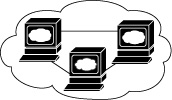
\includegraphics{Cisco_BW/web_cluster}};

\draw[loosely dotted] (LB1) -> (LB2) node[fill=white,midway]{heatbeat};
\draw[dashed] (Internet) -> (LB2);
\draw[dashed] (LB2) -> (farm);

\node [
	start branch=1 going below right,
	diagram item,
	label=below:Other interface
] {\includegraphics{Cisco_BW/PC}};

\node [
	start branch=1 going below left,
	diagram item,
	label=below:Http interface
] {\includegraphics{Cisco_BW/PC}};

\node [
	continue chain = going below,
	diagram item,
	label=below:Modbus interface
] {\includegraphics{Cisco_BW/PC}};

\end{tikzpicture}}
	\scalebox{0.7}{\begin{tikzpicture}[
start chain=going right,
diagram item/.style={
	minimum width=80pt,
	on chain,
	join
},
diagram item seperated/.style={
	minimum width=90pt,
	on chain
}]

\node [
diagram item,
label=above:Client 1
] (client1) {\includegraphics{Cisco_BW/PC}};

\node [
start branch=1 going right,
diagram item seperated,
label=above:Client 2
] (client2){\includegraphics{Cisco_BW/PC}};

\node [
continue branch=1 going right,
diagram item seperated,
label=above:Client 3
] (client3) {\includegraphics{Cisco_BW/PC}};

\node [
continue chain=going below right,
diagram item,
label=center:Internet
] (Internet) {
\includegraphics{Cisco_BW/cloud}};

\node [
start branch=1 going below right,
diagram item seperated,
label={[align=center]right:Load\\Balancer\\(Secondary)}
] (LB2) {
\includegraphics{Cisco_BW/distributed_director}};

\node [
continue chain=going below left,
diagram item,
label={[align=center]left:Load\\Balancer\\(Primary)}
] (LB1) {
\includegraphics{Cisco_BW/distributed_director}};

\node [
continue chain = going below right,
diagram item
] (farm) {};

\node [
start branch=1 going below right,
diagram item,
label=below:Client 3 Handler
] {\includegraphics{Cisco_BW/PC}};

\node [
start branch=1 going below left,
diagram item,
label=below:Client 1 Handler
] {\includegraphics{Cisco_BW/PC}};

\node [
continue chain = going below,
diagram item,
label=below:Client 2 Handler
] {\includegraphics{Cisco_BW/PC}};

%Lines to/from LB2
\draw[loosely dotted] (LB1) -> (LB2) node[fill=white,midway]{heatbeat};
\draw[dashed] (Internet) -> (LB2);
\draw[dashed] (LB2) -> (farm);

\draw (Internet) -> (client2);
\draw (Internet) -> (client3);


\end{tikzpicture}
}
	\captionsetup{format=plain,font=footnotesize,labelfont={bf,defaultCapFont},labelsep=quad,singlelinecheck=no}
	\caption[Distributed system with two load balancing turbines]{
		\label{fig:loadBalancingSetup2Balancers} 
		\footnotesize{%
			A distributed system with two load balancing turbines.
		}
	}
\end{figure}


\paragraph{Single entry point}
Providing a single entry point is simple assigning a static ip address to a turbine would do that, however this introduces a single point of failure.
To overcome this the load balancer must be supplemented by at least one backup load balancer, it must be able to takeover the address of the failing load balancer in order to keep the wind farm available.
This can be done using a virtual ip address, and having the node with the active load balancer respond to it.
If the node with the active load balancer fails the virtual ip address can be transferred to a backup load balancer and it will then become the active load balancer. To let other network participant know that the ip has moved to a new address a ARP announcement can be sent allowing them to update their ARP cache.

\paragraph{Detecting node failure}
Detection of a failed load balancer must be done by the backup nodes, generally there are two ways this can be done, either actively pinging the active load balancer or having the load balancer periodically sent data package also know as heartbeats. This setup is illustrated in \cref{fig:loadBalancingSetup2Balancers}.


\paragraph{Load balancer to server communication}
The key objective of a load balancer is connecting clients to servers. In a basic load balancer this involves keeping track of active connections and transfer packages to the correct server. 

\begin{figure}
	\centering
	\scalebox{0.7}{\begin{tikzpicture}[
start chain=going right,
diagram item/.style={
	minimum width=80pt,
	on chain,
	join
},
diagram item seperated/.style={
	minimum width=90pt,
	on chain
},
arrow/.style={
	->,
	thick,
	shorten <=2pt,
	shorten >=2pt,
},
every join/.style={arrow}
]


\newcommand\millFigure{
\includegraphics[width=0.79cm]{MillSiluet}}

\node [
diagram item,
label=above:Client 1
] (client) {
\includegraphics{Cisco_BW/pc}};


\node [
continue chain=going below right,
diagram item,
label={[align=center]above:Load\\Balancer}
] {\millFigure 
\includegraphics{Cisco_BW/distributed_director}};


\node [
continue chain = going above right,
diagram item,
label={[align=center]above:server}
] (server) {\millFigure};

\draw[arrow] (server) -> (client);
%\draw[arrow] (server.170) -> (client.10);
%\draw[arrow] (client.350) -> (server.190);



\end{tikzpicture}}
	\scalebox{0.7}{\begin{tikzpicture}[
start chain=going right,
diagram item/.style={
	minimum width=80pt,
	on chain,
	join
},
diagram item seperated/.style={
	minimum width=90pt,
	on chain
},
arrow/.style={
	->,
	thick,
	shorten <=2pt,
	shorten >=2pt,
},
every join/.style={arrow}
]


\newcommand\millFigure{
\includegraphics[width=0.79cm]{MillSiluet}}

\node [
diagram item,
label=above:Client 1
] (client) {
\includegraphics{Cisco_BW/pc}};


\node [
continue chain=going below right,
diagram item,
label={[align=center]above:Load\\Balancer}
] {\millFigure 
\includegraphics{Cisco_BW/distributed_director}};


\node [
continue chain = going above right,
diagram item,
label={[align=center]above:server}
] (server) {\millFigure};

\draw[arrow] (server) -> (client);
%\draw[arrow] (server.170) -> (client.10);
%\draw[arrow] (client.350) -> (server.190);



\end{tikzpicture}}
	\captionsetup{format=plain,font=footnotesize,labelfont={bf,defaultCapFont},labelsep=quad,singlelinecheck=no}
	\caption[Load balancer data transportation]{
		\label{fig:LoadbalancerOperation} 
		\footnotesize{%
			Load balancer data transportation.
		}
	}
\end{figure}


\paragraph{Control algorithms} %DNS Datacenter Application
There are multiple ways to distribute traffic that could apply to a decentralized solution.
%Load balancing can be done taking into account many parameters from a simply passing packets to servers in a round robin pattern, to monitoring performance parameters of the servers selecting the one with most free capacity. Some load balancers even inspect packages e.g. pass the HTTP headers URL field to select a server responsible for a specific resource.
Solutions that require client integration or is made for entirely different purposes are omitted as they do not apply to this situation.
Here are some existing strategies:
\begin{enumerate}
	\item Round robin (OSI Layer 2 or 3)
	\item Least-Connection (OSI Layer 2 or 3)
	\item Package inspection (OSI Layer 7)
	\item Performance monitoring
\end{enumerate}

Round robin as the name implies distributes connections to servers equally to each server, it is the most basic of the strategies discussed. In many situations this is will give fair distribution of workload, however this is only true if connecting clients require equal amount of data per connection. If the system has a asymetric load round robin can provide a unfair distribution of workload. 
Round robin has the least overhead.

Least-Connection

Package inspection opens up the package and passes higher protocol headers. This could for instance be HTTP headers in order to identify what service the URL is trying to connect to.
It also makes it possible to split services up in slow and fast running services, helping to make sure that services which need to be fast are not begin slowed down by services which needs to make data heavy calculations.
Doing this would still allow having other distribution strategies to further split up the workload.
Doing package inspection uses more Processing time on the load balancer than the other options since the it needs to process multiple layers of network abstraction to get to the relevant information. In the OSI-model the ip address is defined in layer 3 and the HTTP and Modbus protocols are both part of the application layer and in Layer 7. 

Performance monitoring adds overhead by the added network packages and keeping tack of the current performance of the servers. It however ensure that the server with the most free capacity will receive the connection. Free capacity can be defined as free processing time, available memory or another resource.


\paragraph{Extra Features}

% % % %%SingleEntryPoint and List:LB:LoadBalFailover % % % % % % % %
%The systems needs to respond to a single external IP address. To do this multiple nodes share the same IP address, multiple protocols exists which can do this "Common Address Redundancy Protocol\todo{https://www.freebsd.org/doc/handbook/carp.html}, Virtual Router Redundancy Protocol\todo{http://tools.ietf.org/html/rfc2338} and \cite{zhang2000linuxVirtualServer}".\todo{Put in refferences instead} To provide seamless transfer of the virtual ip address ARP announcements are used to inform the local network of the transfer.
%The backup load balancer monitors the active load balancer and will takeover the virtual ip when the Active load balancer is unavailable and itself become primary this is illustrated in \cref{fig:loadBalancingSetup2Balancers}, this monitoring can be done with the active client sending out periodic heartbeats, or the backup sending ICMP ECHO\_REQUEST.
%Property \ref{List:LB:DetectFailedNodes} requires the load balancer to monitor local nodes for availability, this is to ensure that client connections are not being redirected to a faulty node. This is most easily achived with a ICMP ECHO\_REQUEST otherwise known as a ping request, 


A candidate for this kind of monitoring is the Linux Virtual Server project \cite{zhang2000linuxVirtualServer}.



At a lower tier it could be machine level based on performance parameters like , and finally application level based on the content of the request \textbf{[?]}. %\cite{Citation is missing and I need to find it}.
There exists a lot of solution specific load balancers.
A node balancer is a service which distributes incoming requests, among the services registered on the network.
The distribution is based on different policies like dividing packages or picking the one with most free CPU capacity.
The load balancer could be a single point of failure, it should for this reason always have one or more backups as seen in \cref{fig:loadBalancingSetup}.
The load balancer monitors the real servers and only parses on requests to running servers.
A secondary needs to monitor the primary load balancer and step in if it stops responding.
This can be done using a virtual private IP, which is the address for all incoming requests. Also there exists solutions which does all this in a completely distributed manner avoiding having a central server as load balancer  \textbf{[?]}, %\cite{Some cite I ahven't found yet}, 
this is even in some cases extended to include the clients in the act of load balancing \textbf{[?]}. % \cite{Some cite to netflix eureka balancer}.

In this solution the load balancer needs to balance external connections to different protocols like HTTP and Modbus, however a solution which can be extended to any restful protocol is needed.
Also balancing of node roles depending on the amount incoming traffic on different interfaces will be needed.
Should all this be done automatically or is it better to define this manually???

Load balances can provide various features, related to offloading the real server and node management. % SSL decryprtion, caching, authentication, ...



\begin{figure}
	\centering
	\scalebox{0.7}{\begin{tikzpicture}[
start chain=going right,
diagram item/.style={
	minimum width=30pt,
	on chain
%	join
},
connection/.style={
%	->,
	thick,
	shorten <=2pt,
	shorten >=2pt,
}]

\newcounter{TurbnieCounter}

\newcommand\millFigure{
\includegraphics[width=0.5cm]{MillSiluet}}


\newcommand{\printTurbineID}{\ifnum\value{TurbnieCounter}<10 0\fi\arabic{TurbnieCounter}}
\stepcounter{TurbnieCounter}

\node [
diagram item,
label={[align=center]above:T\printTurbineID\\Load Balancer Active}
] (CenterNode) {\millFigure};
\stepcounter{TurbnieCounter}

\node [
draw,
below =2cm of CenterNode,
inner sep=0.5cm
%label={[align=center]left:T\printTurbineID\\LoadBalancer\\Primary}
] (Switch) {switch};
\draw[connection] (Switch) -- (CenterNode);


\node [
continue chain = going right,
diagram item,
label={[align=center]above:T\printTurbineID\\Spare}
] (Turbine) {\millFigure};
\stepcounter{TurbnieCounter}
\draw[connection] (Switch) -- (Turbine);

\node [
continue chain = going right,
diagram item,
label={[align=center]right:T\printTurbineID\\Spare}
] (Turbine) {\millFigure};
\stepcounter{TurbnieCounter}
\draw[connection] (Switch) -- (Turbine);

\node [
continue chain = going below,
diagram item,
label={[align=center]right:T\printTurbineID\\Spare}
] (Turbine) {\millFigure};
\stepcounter{TurbnieCounter}
\draw[connection] (Switch) -- (Turbine);

\node [
continue chain = going below,
diagram item,
label={[align=center]right:T\printTurbineID\\External\\Interface}
] (Turbine) {\millFigure};
\stepcounter{TurbnieCounter}
\draw[connection] (Switch) -- (Turbine);

\node [
continue chain = going below,
diagram item,
label={[align=center]right:T\printTurbineID\\Spare}
] (Turbine) {\millFigure};
\stepcounter{TurbnieCounter}
\draw[connection] (Switch) -- (Turbine);

\node [
continue chain = going left,
diagram item,
label={[align=center]below:T\printTurbineID\\Spare}
] (Turbine) {\millFigure};
\stepcounter{TurbnieCounter}
\draw[connection] (Switch) -- (Turbine);

\node [
continue chain = going left,
diagram item,
label={[align=center]below:T\printTurbineID\\Spare}
] (Turbine) {\millFigure};
\stepcounter{TurbnieCounter}
\draw[connection] (Switch) -- (Turbine);

\node [
continue chain = going left,
diagram item,
label={[align=center]below:T\printTurbineID\\Spare}
] (Turbine) {\millFigure};
\stepcounter{TurbnieCounter}
\draw[connection] (Switch) -- (Turbine);

\node [
continue chain = going left,
diagram item,
label={[align=center]left:T\printTurbineID\\Spare}
] (Turbine) {\millFigure};
\stepcounter{TurbnieCounter}
\draw[connection] (Switch) -- (Turbine);

\node [
continue chain = going above,
diagram item,
label={[align=center]left:T\printTurbineID\\Spare}
] (Turbine) {\millFigure};
\stepcounter{TurbnieCounter}
\draw[connection] (Switch) -- (Turbine);

\node [
continue chain = going above,
diagram item,
label={[align=center]left:T\printTurbineID\\Sparey}
] (Turbine) {\millFigure};
\stepcounter{TurbnieCounter}
\draw[connection] (Switch) -- (Turbine);

\node [
continue chain = going above,
diagram item,
label={[align=center]left:T\printTurbineID\\Spare}
] (Turbine) {\millFigure};
\stepcounter{TurbnieCounter}
\draw[connection] (Switch) -- (Turbine);

\node [
continue chain = going right,
diagram item,
label={[align=center]above:T\printTurbineID\\Spare}
] (Turbine) {\millFigure};
\stepcounter{TurbnieCounter}
\draw[connection] (Switch) -- (Turbine);



%\node [
%continue chain = going below,
%diagram item,	
%label={[align=center]right:T04\\LoadBalancer\\Primary}
%] (end1) {\millFigure};

%\draw (endBranch1) -> (end1) node{};
%\draw (endBranch1) -> (startBranch) node{};
%\draw (endBranch1) -> (start) node{};
%\draw (end1) -> (startBranch) node{};



%\draw (endBranch2) -> (end2) node{};

\end{tikzpicture}}
	\captionsetup{format=plain,font=footnotesize,labelfont={bf,defaultCapFont},labelsep=quad,singlelinecheck=no}
	\caption[System overview from the load balancer viewpoint]{
		\label{fig:parkOverview} 
		\footnotesize{%
			A system overview of park nodes.
		}
	}
\end{figure}

 
%\paragraph{consider the} 
%\begin{itemize}
%\item job migration cost
%\item resource heterogeneity
%\item network heterogeneity
%
%\item resource usage
%\item conditions
%\end{itemize}
%
%\paragraph{performance parameters}
%\begin{itemize}
%\item job size
%\item data transfer rate
%\item status exchange period
%\item migration limit
%\end{itemize}

%\paragraph{Algorithms/policies}
%\begin{itemize}
%	%(On the Design of Adaptive and Decentralized	Load-Balancing Algorithms with Load Estimation for Computational Grid Environments)	
%	\item MELISA Modified ELISA (used for large scale system (interGrid))
%	\item LBA Load Balancing on Arrival
%	
%	\item Round-robin (Weighted/unweighed)
%	\item Least-Connection (Weighted/unweighed)
%\end{itemize}
%
%\paragraph{The following requirements to the system exists}
%\begin{itemize}
%	\item Robustness
%	\item Protocol flexible
%	\item Must be a distributed component
%\end{itemize}
%
%\paragraph{Preferred features}
%\begin{itemize}
%	\item support TCP Handoffs (for non restful applications)
%\end{itemize}
%
%\subsection{Levels of balancing}
%\begin{description}
%	\item[??] DDNS / Round robin DNS
%	\item[OSI 3] Network/IP %google says network layer LVS says transport layer
%	\item[OSI 4] Network/IP
%	\item[OSI 7] {Application level, like http balancing, allows balancing strategies based on url and user location.}
%\end{description}
%
%What we would like is a transport layer protocol.
%\vspace{1cm}

%\noindent\cite{Ludwig:SwarmIntelligenceGridLoadBalancing} 
%Implements a particle swam based and an ant based algorithm. 
%It discuses quality parameters.
%It compares with a version using distributed knowledge (SBA State Broadcast Algorithm)
%\\

%\noindent\cite{MayuriMehta:HybridDynamicLB} Central and distributed Balancing (hybrid). Central(3) dosn't scale, distributed (6 refs) has a larger overhead. Implements node selection algorithms.
%
%Nice comparison of load balancers
%\url{http://codeghar.wordpress.com/2007/11/04/create-a-load-balance-server-using-ubuntu/}
%
%hearbeat 	\url{http://people.adams.edu/~cdmiller/posts/nginx-heartbeat-ha/}
%
%\url{http://kaivanov.blogspot.dk/2013/01/building-load-balancer-with-lvs-linux.html}
%\url{http://sorrawut.com/lvs-dr/}
%\subsection{Existing solutions}
%\begin{description}
%	\item [Linux Virtual Server: IPVS] Is implemented in the linux kernal version 2.4 and 2.6. Works at the IP level. Used by big sites sourceforge.net, layer 3.
%	\item [Google Compute Engine: Load Balancer]: Proprietary. layer 3 and 7.
%	%http://aws.amazon.com/route53/
%	\item [Amazon Route 53] DNS based server, provides region based balancing and latency balancing.
%	\item [AWS ELB] Amazons load balancer, Proxy based, top tier
%	%https://github.com/Netflix/eureka/wiki/Eureka-at-a-glance
%	\item [Eureka] Netflix Load Balancer, client based, middle tier
%
%	\item [Loadbalancer.org] ...
%	\item [HAProxy] ...
%	\item [pfsense] ...
%	\item [http://www.ultramonkey.org/]
%	\item [Balance] ...
%	\item [Crossroads] ...
%	\item [nginx] \url{http://nginx.org/en/docs/http/load_balancing.html}
%	\item [varnish-cache] \url{https://www.varnish-cache.org/trac/wiki}
%\end{description}

%\begin{itemize}
%	\item batch schedulers
%	\item workflow engines
%	\item operating systems (build in scheduler)
%\end{itemize}

%\begin{figure}
%	\centering	
%	\scalebox{0.7}{\begin{tikzpicture}[
start chain=going right,
diagram item/.style={
	minimum width=80pt,
	on chain,
	join
},
diagram item seperated/.style={
	minimum width=90pt,
	on chain
}]

\node [
diagram item,
label=above:Client 1
] (client1) {\includegraphics{Cisco_BW/PC}};

\node [
start branch=1 going right,
diagram item seperated,
label=above:Client 2
] (client2){\includegraphics{Cisco_BW/PC}};

\node [
continue branch=1 going right,
diagram item seperated,
label=above:Client 3
] (client3) {\includegraphics{Cisco_BW/PC}};

\node [
continue chain=going below right,
diagram item,
label=center:Internet
] (Internet) {
\includegraphics{Cisco_BW/cloud}};

\node [
start branch=1 going below right,
diagram item seperated,
label={[align=center]right:Load\\Balancer\\(Secondary)}
] (LB2) {
\includegraphics{Cisco_BW/distributed_director}};

\node [
continue chain=going below left,
diagram item,
label={[align=center]left:Load\\Balancer\\(Primary)}
] (LB1) {
\includegraphics{Cisco_BW/distributed_director}};

\node [
continue chain = going below right,
diagram item
] (farm) {};

\node [
start branch=1 going below right,
diagram item,
label=below:Client 3 Handler
] {\includegraphics{Cisco_BW/PC}};

\node [
start branch=1 going below left,
diagram item,
label=below:Client 1 Handler
] {\includegraphics{Cisco_BW/PC}};

\node [
continue chain = going below,
diagram item,
label=below:Client 2 Handler
] {\includegraphics{Cisco_BW/PC}};

%Lines to/from LB2
\draw[loosely dotted] (LB1) -> (LB2) node[fill=white,midway]{heatbeat};
\draw[dashed] (Internet) -> (LB2);
\draw[dashed] (LB2) -> (farm);

\draw (Internet) -> (client2);
\draw (Internet) -> (client3);


\end{tikzpicture}
}
%	\captionsetup{format=plain,font=footnotesize,labelfont={bf,defaultCapFont},labelsep=quad,singlelinecheck=no}
%	\caption[Routing requests as load balancing]{
%		\label{fig:RoutingloadBalancingSetup} 
%		\footnotesize{%
%			Routing requests as load balancing.
%		}
%	}
%\end{figure}


% % % SSK Might Be usable later until then hidden here % % %
% % % DNS load balancers are not relevant to the Simens case. % % % %
%Different load balancing methods will are here briefly described:
%%Load balancing for large systems can be split in tiers.
%\paragraph{Dynamic DNS}
%is a load balancer built into the DNS service, it distributes load in a round robin manner as well as using region knowledge of where the request was revived from \cite{Amazon:Route53}. DNS based load balancing is among the most scalable solutions that does not need any special configuration of either client nor server. However is does not provide any monitoring of server performance parameters, and once the DNS lookup is over the service does not play any role in load balancing related to one that specific client until the DNS cache is refreshed. This type of loadbalancing is not applicable since 












